\subsubsection{Trends in Independent Features}\label{sec:impl-data-analysis:independent-features}
The feature transformation based on collinearity factor carried out in Section \ref{sec:impl-data-analysis:corr:generic-approach} has reduced the number of features present in the dataset to 33. The new overall feature correlation statistics have been illustrated in Figure \ref{fig:corr:post-transformation}. From same, a number of independent features, where the correlation factor is close to 0, can be observed.

The first candidate for trend analysis is illustrated in Figure \ref{fig:corr:post-transformation:overallCoverage-complexity-ncloc} and consisted of \overallCoverage{}, \complexity{} and\ncloc{} features. It should be noted that while \ncloc{} and \complexity{} attributes display a strong positive correlation the \overallCoverage{} feature is unrelated to either of the two attributes. The same observation can be made from Figure \ref{fig:corr:post-transformation:overallCoverage-complexity-ncloc} where the metric representing the number of source code lines, \ncloc{}, and the metric representing overall complexity of the code move together. Additionally, despite the lack of strong indication of the collinearity, the overall coverage metric increases in value along with the source code line metric. Taking into the account the domain knowledge of any software development project, the greater the number of the source code lines present the larger the number of code to be covered by test automation. What is interesting in the underlying scenario is that the growth of source code is closely followed by the increase of test automation coverage. 

\begin{figure}[!h]
    \centering
    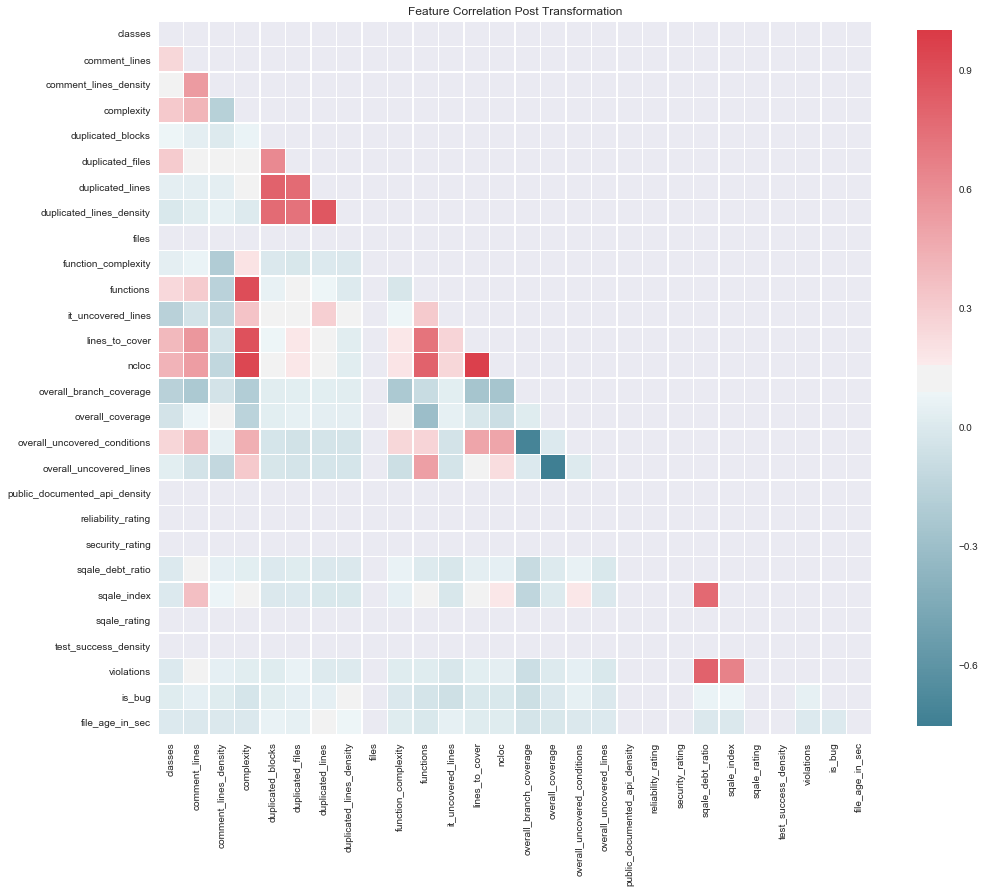
\includegraphics[scale=0.48]{Figures/correlation/Feature_Correlation_Post_Transformation.png}
    \caption{Feature Correlation after Feature Transformation}
    \label{fig:corr:post-transformation}
\end{figure}

\begin{figure}[!h]
    \centering
    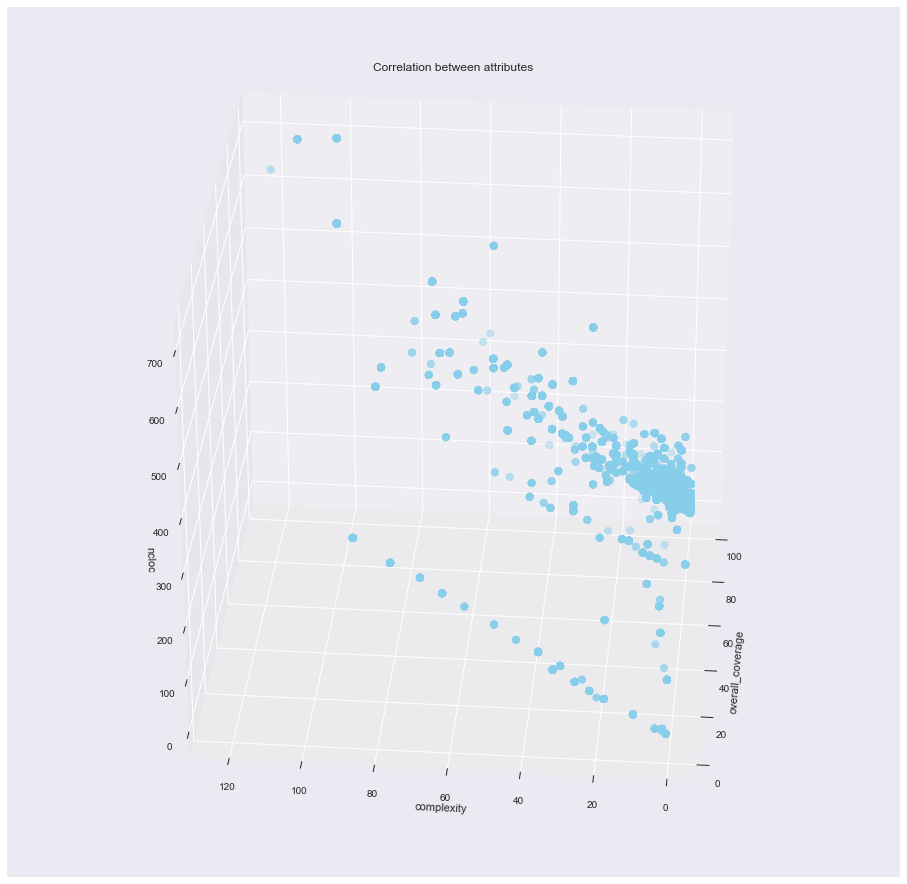
\includegraphics[scale=0.5]{Figures/independent-feat-trends/Correlation_between_attributes_overall_coverage_complexity_ncloc.png}
    \caption{Independent Features Correlation - \overallCoverage{}, \complexity{} and \ncloc{}}
    \label{fig:corr:post-transformation:overallCoverage-complexity-ncloc}
\end{figure}

Another set of independent features is represented by \sqaleIndex{}, \sqaleRating{} and \sqaleDebtRatio{} attributes. Again, while there is little to no collinearity defined between the three attributes, from Figures \ref{fig:corr:post-transformation:sqale} it can be determined that a relationship between feature data exists. The higher the \sqaleIndex{} the higher the value of \sqaleDebtRatio{}. 
\begin{figure}
    \centering
    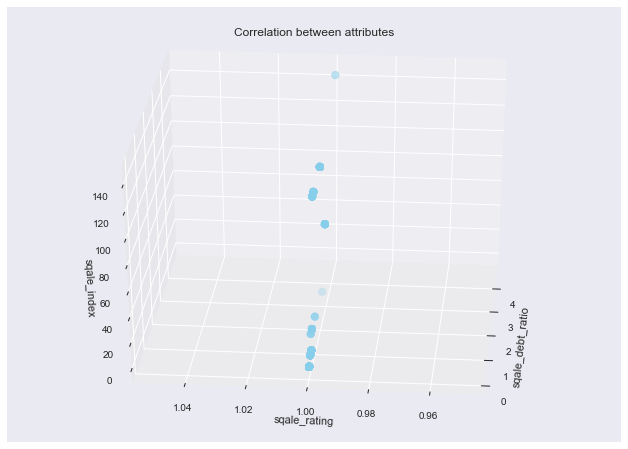
\includegraphics[scale=0.7]{Figures/independent-feat-trends/Correlation_between_attributes_sqale_debt_ratio_sqale_rating_sqale_index.png}
    \caption{Independent Features Correlation - SQALE Metrics}
    \label{fig:corr:post-transformation:sqale}
\end{figure}

The above trend analysis provides a conclusion that not all relationships between data are based on collinearity factor. Instead, some relationships present in the dataset are inherent to the data gathered, as was the case with metrics depicted in Figures \ref{fig:corr:post-transformation:overallCoverage-complexity-ncloc} and \ref{fig:corr:post-transformation:sqale}.
\FloatBarrier